\documentclass[11pt]{ltjsarticle}
\usepackage{amsmath}
\usepackage{amssymb}
\usepackage{amsfonts}
\usepackage{physics}
\usepackage{graphicx}
\usepackage{float}
\usepackage{booktabs}
\usepackage{tikz}
\usepackage{xcolor}
\usepackage{pgfplots}
\usepackage{mathcomp}
\usepackage{enumitem}
\usepackage{wrapfig}
\usepackage{etoolbox}
\usepackage{cleveref}
\crefformat{figure}{図~#2#1#3}  % 図の日本語設定
\crefformat{equation}{式~(#2#1#3)}  % 式の日本語設定
\crefformat{table}{表~#2#1#3}  % 表の日本語設定
\usetikzlibrary{intersections,calc}
\pgfplotsset{compat=1.18}
\begin{document}
  \begin{figure}[H]
    \centering
    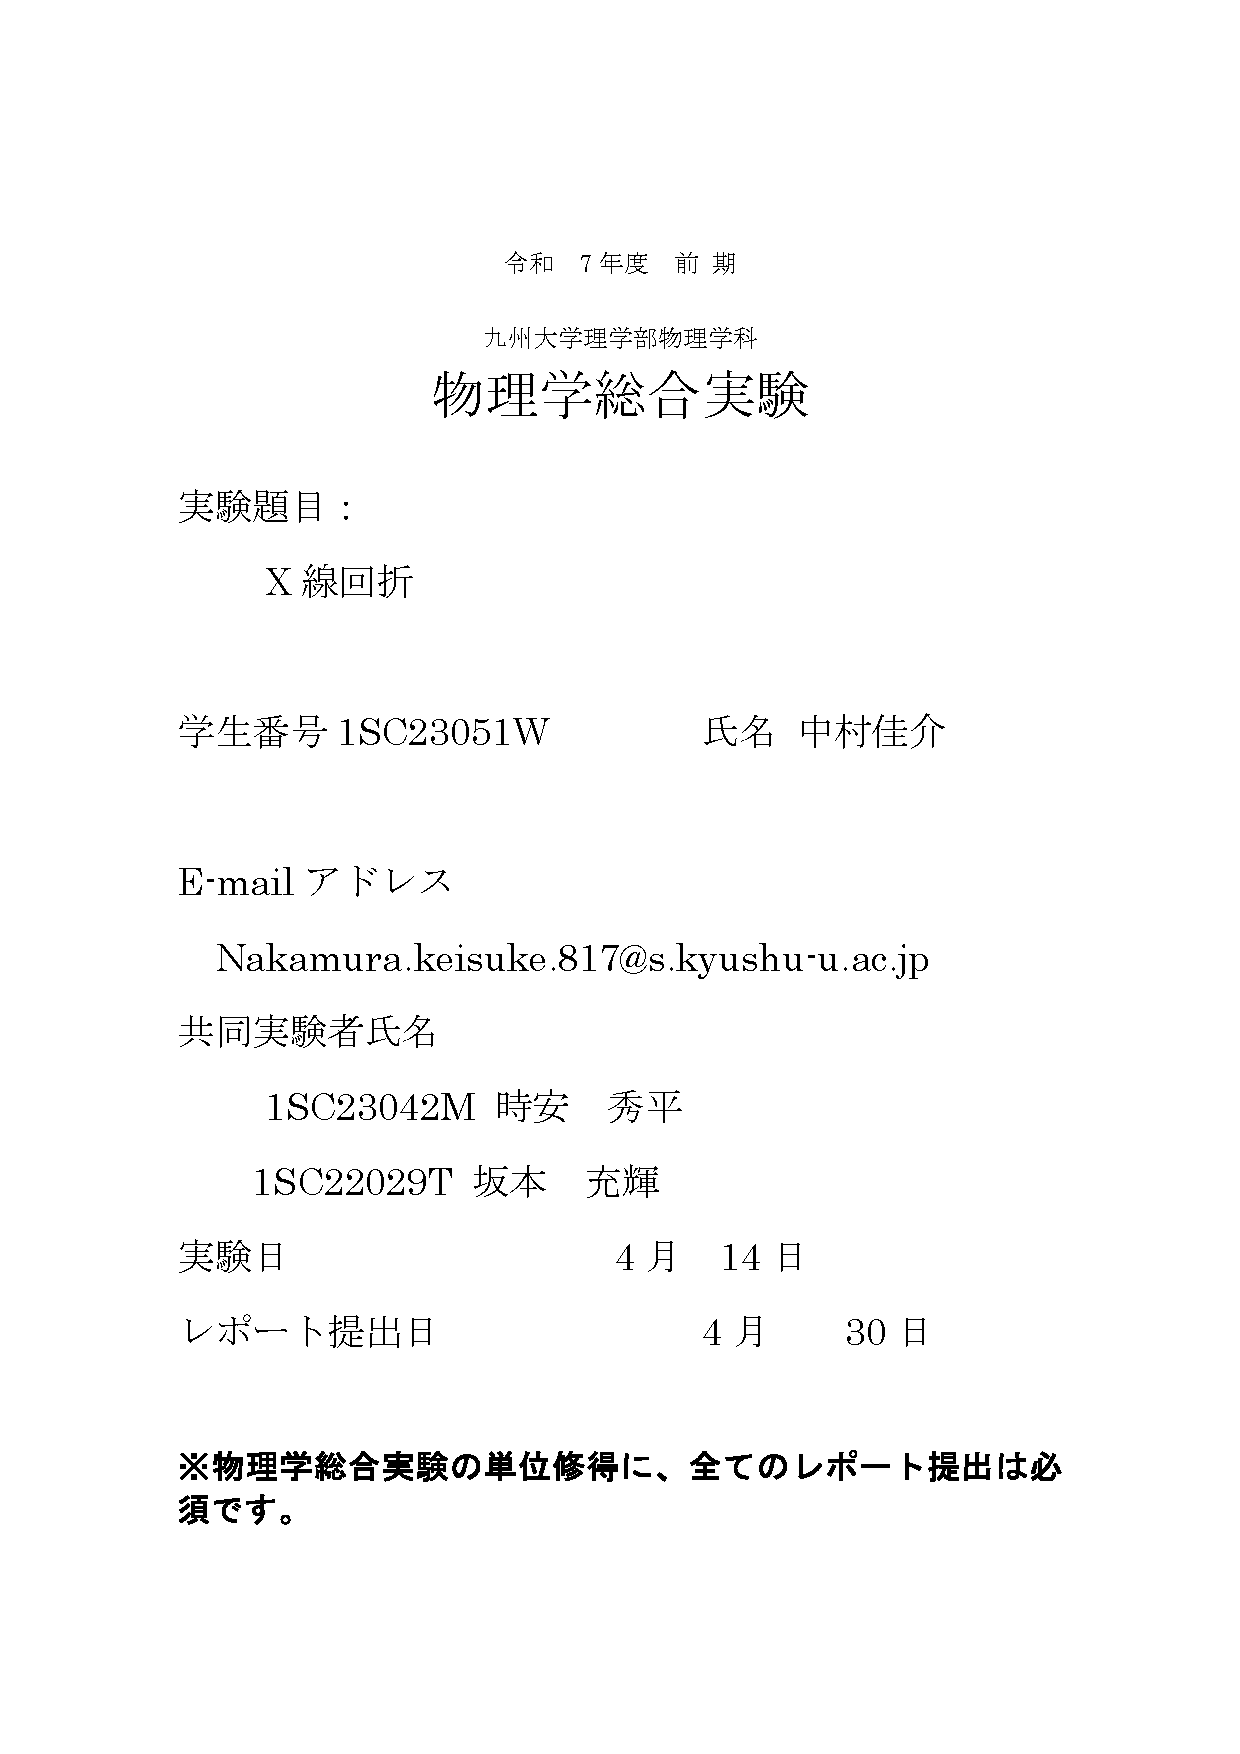
\includegraphics[width=\columnwidth]{hyoushi_xrd.pdf}
  \end{figure}
  
  \section*{目的}
    結晶の原子サイズの構造をX線回折を利用して理解する.
  \section*{原理}
    物質の性質は原子の配列構造によって決まるため, 物質の原子レベルの構造を理解することが物質の性質を理解することにつながる. その方法として原子間距離と同程度の波長を持つX線回折現象が広く用いられている. 
    結晶にX線を照射すると回折像が得られるということが1912年にM.T.F von Laueらにより発見された.  この現象を利用することにより, 結晶の周期配列, 原子構造を理解できる. 
    \subsection*{原子周辺の散乱と回折現象}
    \begin{figure}[H]
      \centering
      % 左側:文章
      \begin{minipage}[t]{0.6\textwidth}
        \vspace{0pt}
        \cref{fig:xrd}のようにX線が結晶中の原子にぶつかると、X線の電場によって原子中の核外電子が振動する。
        すると入射X線と同波長、逆位相の電磁波が原子核を中心として球面上に放射される。
        各原子からの電磁波が干渉し、回折現象が起こる。
      \end{minipage}
      \hfill
      % 右側:図
      \begin{minipage}[t]{0.35\textwidth}
        \vspace{0pt}
        \centering
        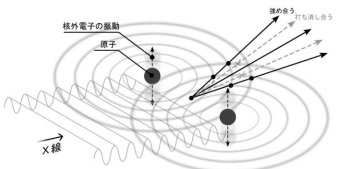
\includegraphics[width=\linewidth]{xrd1.png}
        \caption{結晶中の原子によるX線の散乱, 回折.}
        \label{fig:xrd}
      \end{minipage}
    \end{figure}
    \subsection*{結晶によるX線回折}
    \begin{figure}[H]
      \centering
      % 左側:文章
      \begin{minipage}[t]{0.6\textwidth}
        \vspace{0pt} % ← 上揃えのために必要
        X線回折実験において、X線の入射方向を変えると様々な結晶面からの反射により、結晶構造を調べることができる。\\
        X線回折実験ではX線の入射方向により様々な結晶面からの反射波を得て、それを解析することで結晶構造を調べる。\\
        結晶面を表現するためにミラー指数を導入する。図\ref{fig:mirror}のように、面(hkl)はa軸上の$\vb*{a}/h$, $\vb*{b}/k$, $\vb*{c}/l$を通る平面とする. 
        結晶面(hkl)が$d_{hkl}$の間隔をとって並んでいる状況(図\ref{fig:hansha})を考え, そこにX線(波長\lambda)が入射すると二つのX線の経路差は$2d_{hkl}\sin{\theta}$となる.
        このとき, 
        \begin{gather}
          2d_{hkl}\sin{\theta}=n\lambda
          \label{eq:bragg}
        \end{gather}
        というブラッグの条件が成り立てば反射光同士は強めあう. しかしすべての結晶面から回折がみられるわけではなく, (hkl)面からのX線の回折強度は以下で与えられる.
        \begin{gather}
          \text{回折X線強度:}I(k)=s|F(hkl)|^2\\
          \text{構造因子:}=\sum_{j}^{} f_j \exp{2\pi i(hx_j +ky_j +lz_j)}
        \end{gather}
        ここで$f_j$は原子散乱因子であり, 原子一個からの散乱を特徴づけるものである. 
        また, 式(3)は構造因子と呼ばれる単位格子からの散乱波の振幅である.実験の際は式(2)のように散乱因子の二乗に比例する回折強度を測定する. sは実験の条件を補正する係数である. 
      \end{minipage}
      \hfill
      % 右側:図
      \begin{minipage}[t]{0.35\textwidth}
        \vspace{0pt}
        \centering
        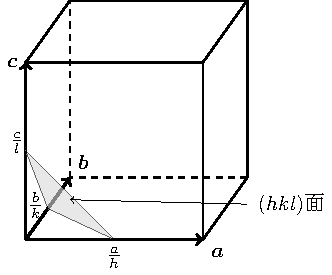
\includegraphics[width=\linewidth]{xrd_figure1.pdf}
        \caption{ミラー指数による結晶面の表現}
        \label{fig:mirror}
        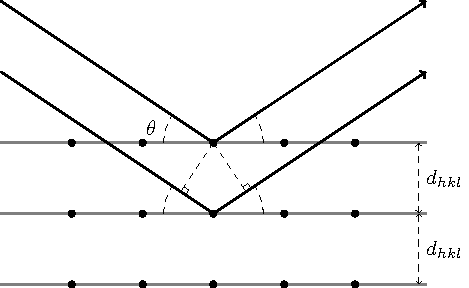
\includegraphics[width=\linewidth]{xrd_figure2.pdf}
        \caption{結晶面からのブラッグ反射}
        \label{fig:hansha}
      \end{minipage}
    \end{figure}
    \subsection*{実施した実験の個別の計算}
      今回実施した実験における構造因子を求めてみる.
      今回, 実験にはアルミニウム(Al)を使用した. アルミニウムの結晶構造は面心立方格子であり, その単位格子に4つの格子点\\
      $(x,y,z)=(0,0,0),(0,\frac{1}{2},\frac{1}{2}),(\frac{1}{2},0,\frac{1}{2}),(\frac{1}{2},\frac{1}{2},0)$
      が存在し, 式(3)にこれを代入すると, 
      \begin{gather}
        F(hkl)=f \{1+\exp[i\pi (h+k)]+\exp[i\pi (k+l)]+\exp[i\pi (l+h)]\}
      \end{gather}
      が得られる.
      なお, 原子はすべてAlであるため$f_j =f$としている. 式(4)よりアルミニウムの場合, h,k,lがすべて奇数, またはすべて偶数の場合に$F(hkl)\not= 0$となる.
  \section*{実験}
    \subsection*{X線の発生}
      X線発生には{\cref{fig:xrayapper}}のような装置を用いる. フィラメントを熱し, 熱電子を飛び出させ, 高電圧により加速して金属ターゲットに衝突させることによりX線を発生させる. 
      このとき, 金属ターゲットから連続X線と特性X線の二種類が放出される. 連続X線は金属ターゲットに電子がぶつかる際に減速し, 連続的に分布し, 白色のX線になる. 特性X線は入射電子が金属ターゲットの電子を励起できるようなエネルギーがあるとき, 空いたホールに高エネルギー準位から電子が落ち込み, そのエネルギー差からX線が放出される. このX線はターゲットの金属原子の種類によって固有の波長を持つ. このX線を特性X線と呼ぶ. 
      今回の実験では$\mathrm{Cu}K\alpha$線($\lambda(K\alpha_1)={1.5405}{\text{\AA}},\lambda(K\alpha_2)={1.5443}\text{\AA})$を用いた.
      \begin{figure}[H]
        \centering
        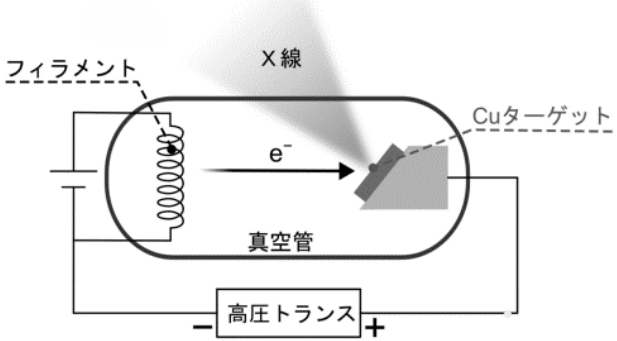
\includegraphics[width=0.4\columnwidth]{xrayapper.png}
        \caption{X線の発生}
        \label{fig:xrayapper}
      \end{figure}
    \subsection*{実験装置}
    \begin{minipage}[b]{0.45\textwidth}
      \begin{figure}[H]
        \centering
        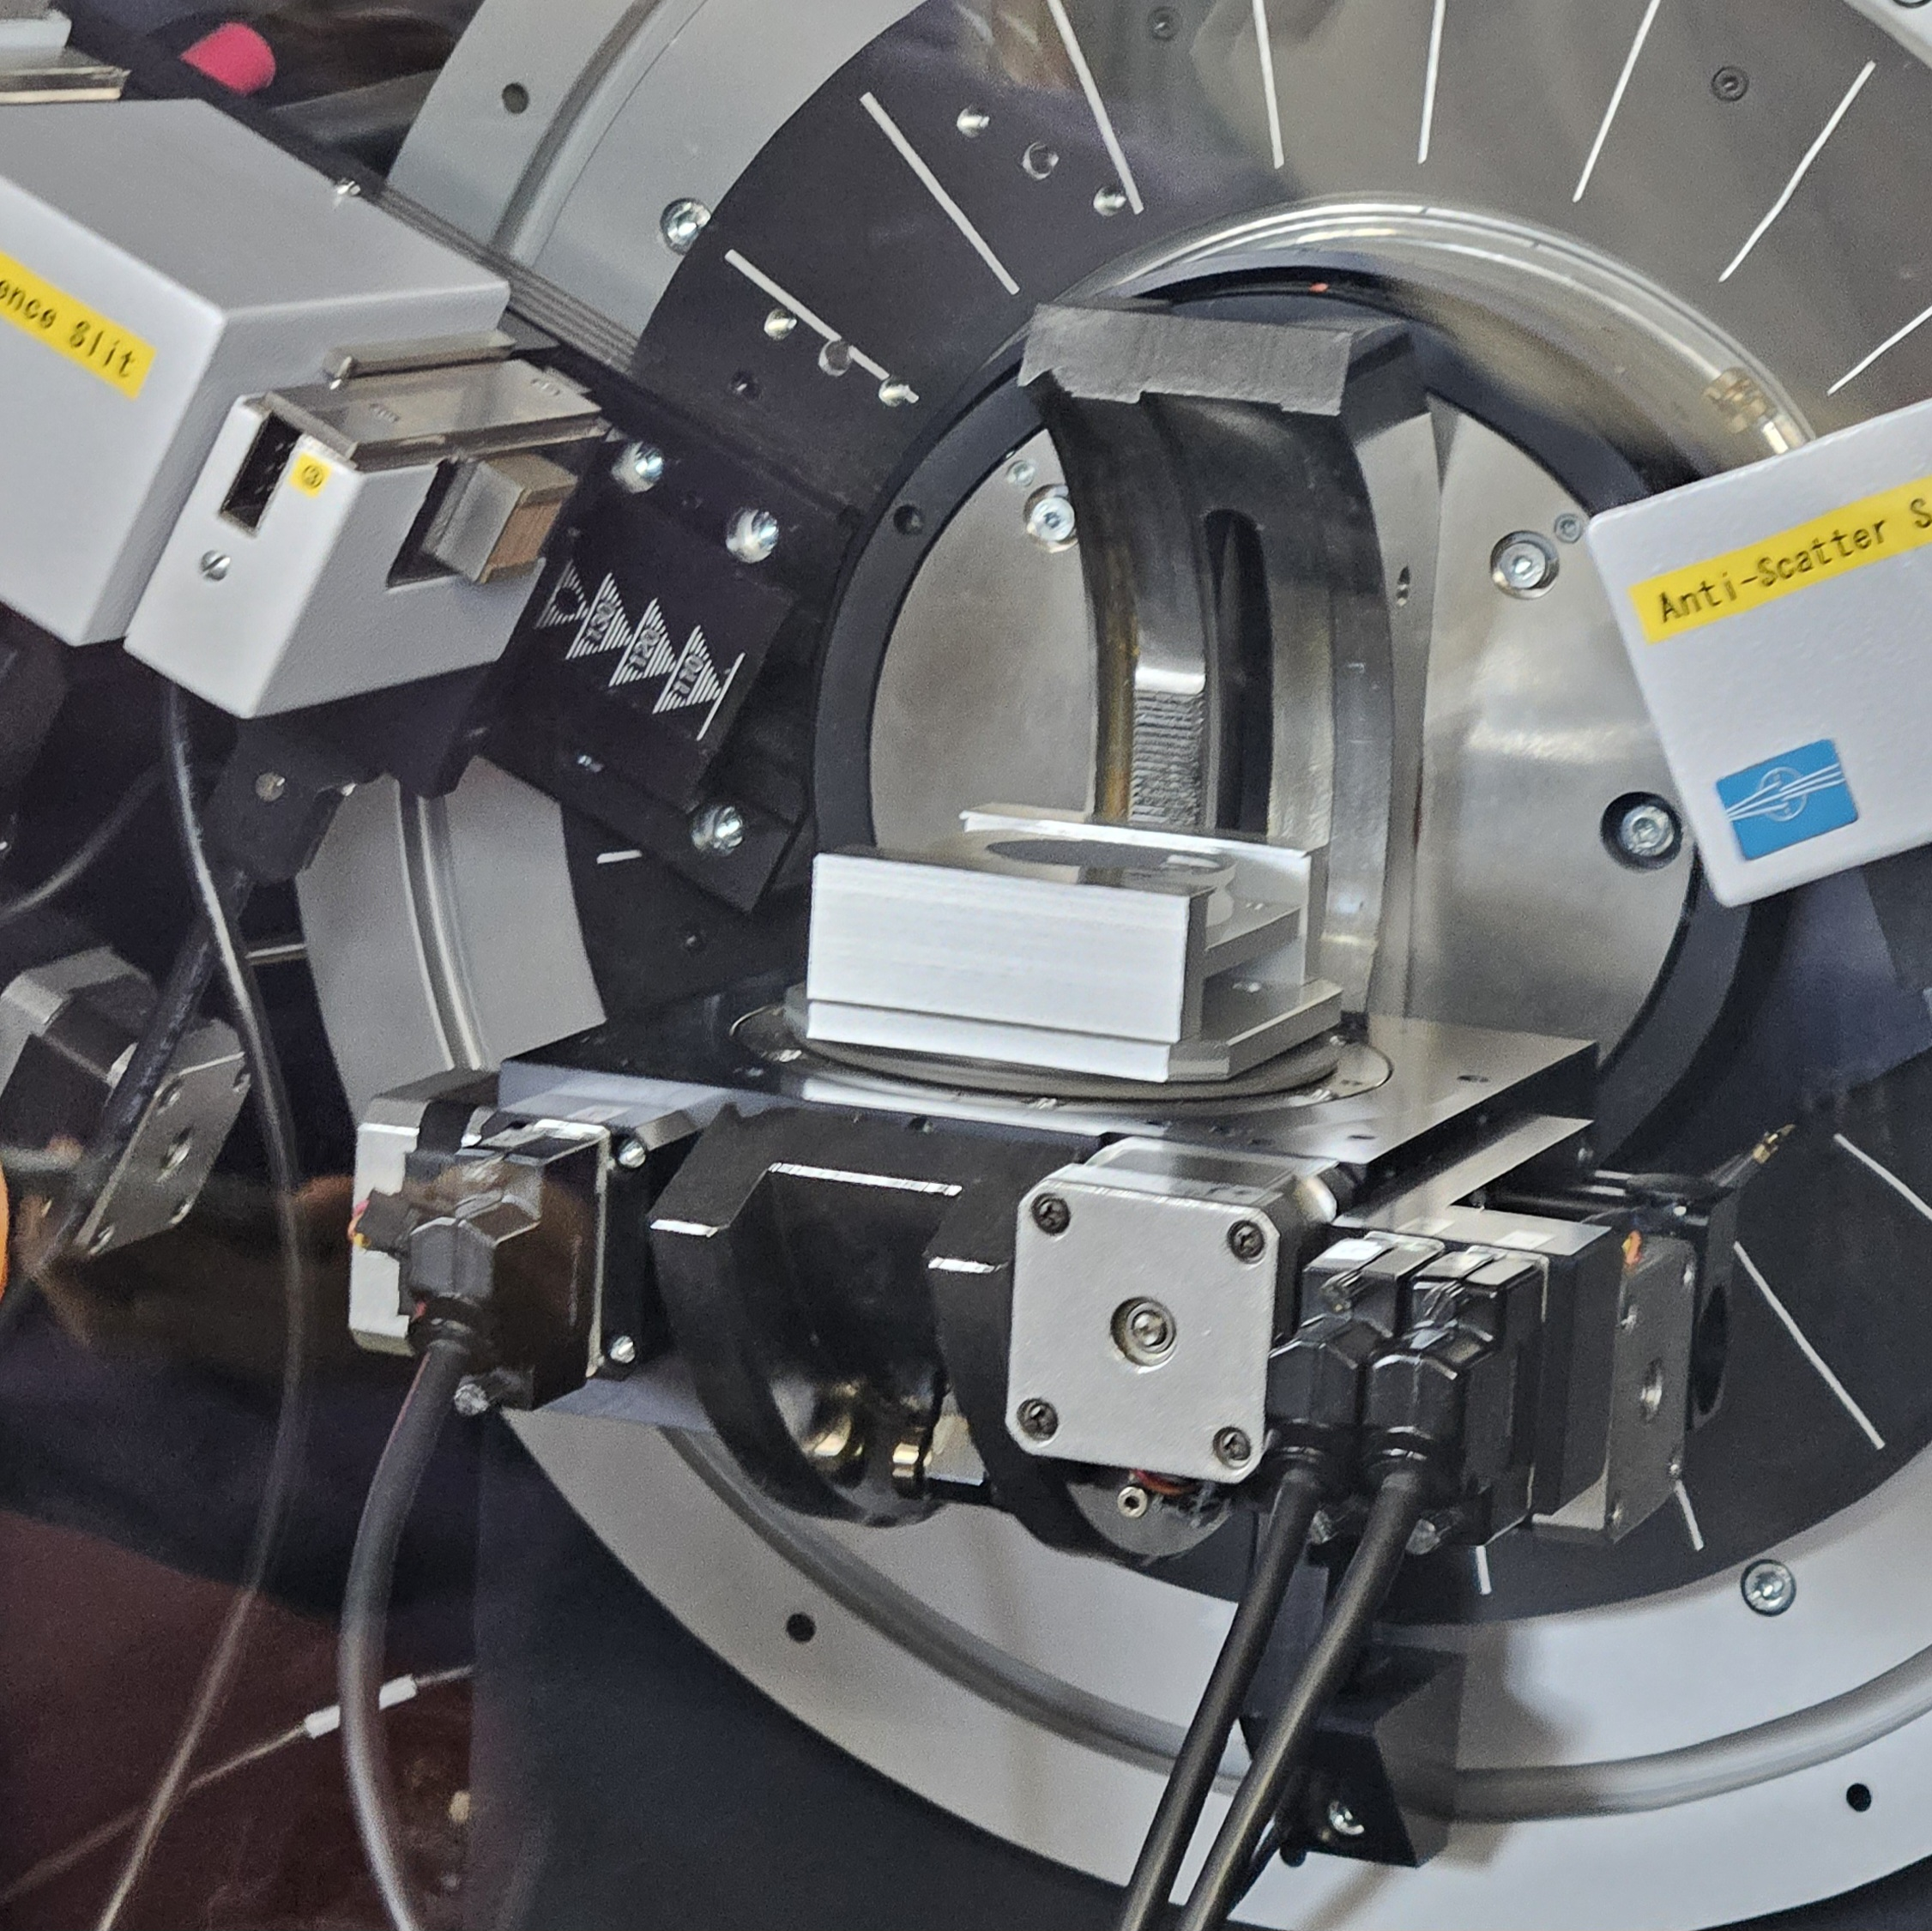
\includegraphics[width=0.97\columnwidth]{jikkenkigu.jpg}
        \caption{実験装置}
        \label{fig:jikkenkigu}
      \end{figure}
    \end{minipage}
    \hfill
    \begin{minipage}[b]{0.45\textwidth}
      \vfill
      \begin{figure}[H]
        \centering
        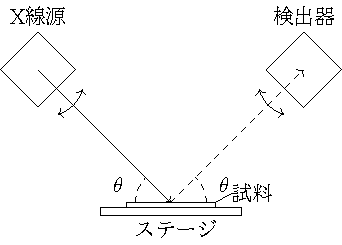
\includegraphics[width=\columnwidth]{xrd_figure3.pdf}
        \caption{実験装置模式図}
        \label{fig:moshiki}
      \end{figure}
    \end{minipage}
    \\
    装置は\cref{fig:moshiki}のようにX線源と検出器が動き, あらゆる角度からサンプルにX線を照射することができるようになっている.
    \subsection*{測定手順}
      \begin{enumerate}
        \item X線源のシャッターが閉じていることを確認し, 装置のドアを開け, Al板をステージに固定した. 
        \item ここで測定の設定を$2\theta =20^{\circ}$から$2\theta =100.0354^{\circ}$, $2\theta=0.01539^\circ$刻みにし, PSD opening(検出器のスリットの開き具合)は$2.9397^\circ$で測定を開始した.
        \item X線源のシャッターが閉じていることを確認して装置のドアを開け, Al板をステージから回収した. 
      \end{enumerate}
  \section*{結果}
    \subsection*{課題1}
      \begin{enumerate}
        \item (4)式の右辺をfccと置くと, Siの構造因子は
          \begin{gather}
            F'(hkl)=\text{fcc}\{1+\exp[\frac{\pi}{2}i(h+k+l)]\}
          \end{gather}
          のようになり, $F'(hkl)\neq 0$であるには, fccの条件であるh, k, lがすべて奇数,またはすべて偶数の条件を満たし, $h+k+l \not\equiv 2 (\bmod 4)$
          を同時に満たす必要がある.
        \item あるベクトル$\vb*{G}=h \vb*{x}+k \vb*{y}+l \vb*{z}$を考える.立方晶であることより$\vb*{x}\cdot \vb*{y}=\vb*{x}\cdot\vb*{z}, |\vb*{x}|=|\vb*{y}|=|\vb*{z}|$が成立する.
          \begin{gather}
            \vb*{G} \cdot \qty(\frac{\vb*{x}}{h}-\frac{\vb*{y}}{k})=\vb*{G}\cdot \qty(\frac{\vb*{x}}{h}-\frac{\vb*{z}}{l})=0
            \label{eq:cross}
          \end{gather}
          \cref{eq:cross}において$\frac{\vb*{x}}{h}-\frac{\vb*{y}}{k}, \frac{\vb*{x}}{h}-\frac{\vb*{z}}{l}$はどちらも面hkl上のベクトルであるので, $\vb*{G}$は面hklと直行する. \\
          したがって原点からG方向に$d_{hkl}$進んだベクトルは$\frac{\vb*{x}}{h}$を$\vb*{G}$が定める直線に正射影したベクトルであるので式(7)が成立.\\
          \begin{gather}
            d_{hkl}\frac{\vb*{G}}{|\vb*{G}|}=\frac{1}{h}\frac{\vb*{G}\cdot \vb*{x}}{|\vb*{G}|^2}\vb*{G}\\
            d=\frac{1}{h}\frac{\vb*{G}\cdot \vb*{x}}{|\vb*{G}|}\notag\\
            d=\frac{a}{|\vb*{G}|}\notag\\
            d=\frac{a}{\sqrt{h^2 +k^2 +l^2}}
            \label{eq:mirror}
          \end{gather}
          \cref{eq:mirror}より,$1/d_{hkl}^2 =(h^2 +k^2 +l^2)/a^2$
      \end{enumerate}
    実験結果をグラフにプロットしたものが\cref{fig:xrdgraph1}である. 
    \begin{figure}[H]
      \centering
      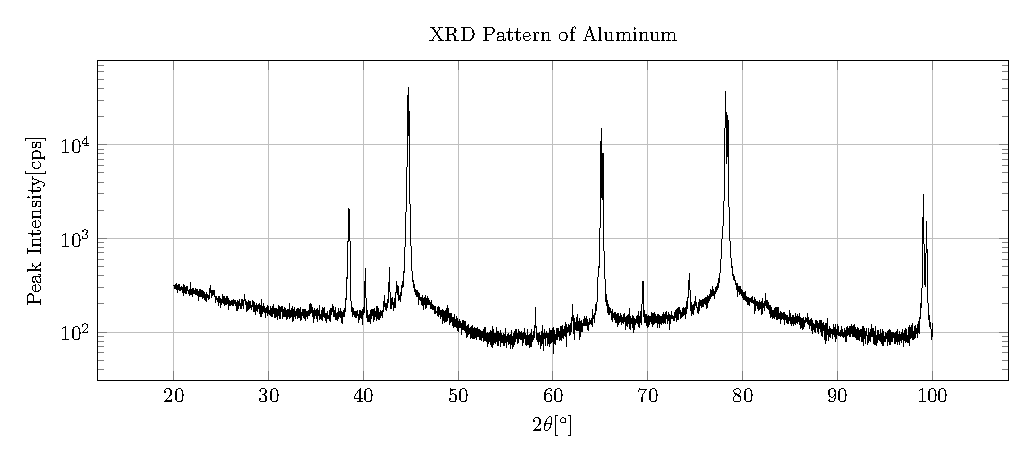
\includegraphics[width=0.98\columnwidth]{xrd_graph1.pdf}
      \caption{測定結果}
      \label{fig:xrdgraph1}
    \end{figure}
    \subsection*{課題2}
      \begin{enumerate}
        \item pythonのNumPy, SciPyライブラリを用いてピークを検出し, \cref{fig:xrdgraph1}にピークを追加したものが\cref{fig:xrdgraph2}である.
          また, 二つのピークが近い(差が$2\theta<0.4^\circ$)ときは低角側のピークのみ抜き出すようにすると\cref{tab:peak}のようになった.
          \begin{figure}[H]
            \centering
            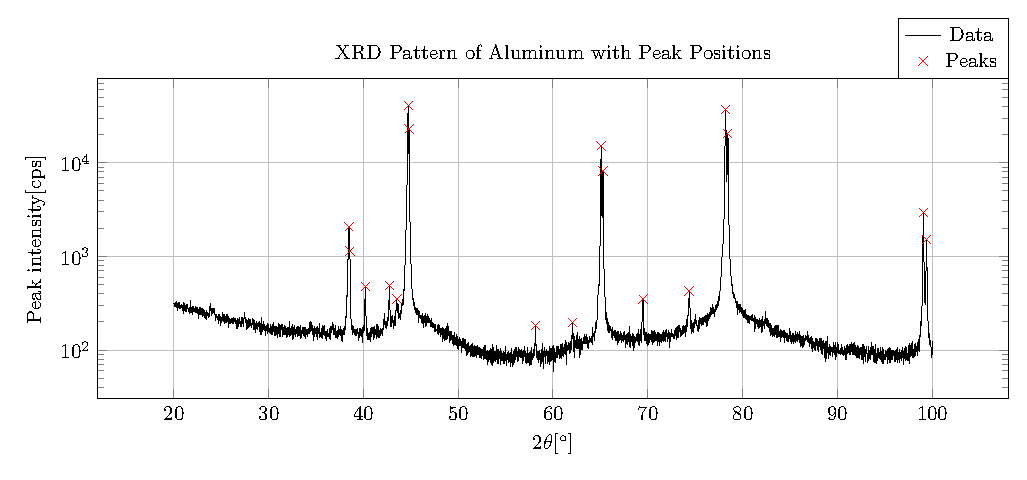
\includegraphics[width=0.7\columnwidth]{xrd_graph2.pdf}
            \caption{ピーク位置}
            \label{fig:xrdgraph2}
          \end{figure}
          
          \begin{table}[ht]
          \centering
          \resizebox{\textwidth}{!}{ % 表の幅をページの幅に合わせてリサイズ
          \begin{tabular}{|c|c|c|c|c|c|c|c|c|c|c|c|c|}
          \hline
          $2\theta[^\circ]$ & 38.4851 & 40.2243 & 42.7639 & 43.5181 & 44.7186 & 58.1707 & 62.0493 & 65.0968 & 69.5142 & 74.3625 & 78.2103 & 99.0657 \\
          \hline
          ピーク強度[cps]& 2087 & 475 & 491 & 351 & 40962 & 184 & 198 & 15157 & 349 & 426 & 37309 & 2939 \\
          \hline
          \end{tabular}
          }
          \caption{ピークのデータ}
          \label{tab:peak}
          \end{table}
        \item \cref{eq:bragg}を用いて各ピークに対応する面間隔dを求めると\cref{tab:menkankaku}のようになった.
          \begin{table}[H]
            \centering
            \resizebox{\columnwidth}{!}{
              \begin{tabular}{|c|c|c|c|c|c|c|c|c|c|c|c|c|}\hline
              $2\theta[^\circ]$ & 38.4851 & 40.2243 & 42.7639 & 43.5181 & 44.7186 & 58.1707 & 62.0493 & 65.0968 & 69.5142 & 74.3625 & 78.2103 & 99.0657 \\
              \hline
              面間隔d[\AA]&2.3372 & 2.2400 & 2.1127 & 2.0778 & 2.0248 & 1.5845 & 1.4945 & 1.4317 & 1.3511 & 1.2745 & 1.2212 & 1.0125 \\
              \hline
              \end{tabular}
            }
            \caption{ピークと面間隔}
            \label{tab:menkankaku}
          \end{table}
        \item 格子定数の比とミラー指数の二乗和を比較してミラー指数を特定すると\cref{tab:mirror}のようになった.
          \begin{table}[H]
            \centering
            \resizebox{\columnwidth}{!}{
              \begin{tabular}{|c|c|c|c|c|c|c|c|c|c|c|c|c|}\hline
              $2\theta[^\circ]$ & 38.4851 & 40.2243 & 42.7639 & 43.5181 & 44.7186 & 58.1707 & 62.0493 & 65.0968 & 69.5142 & 74.3625 & 78.2103 & 99.0657 \\
              \hline
              面間隔d[\AA]&2.3372 & 2.2400 & 2.1127 & 2.0778 & 2.0248 & 1.5845 & 1.4945 & 1.4317 & 1.3511 & 1.2745 & 1.2212 & 1.0125 \\
              \hline
              ミラー指数(h,k,l)&(1,1,1)&ノイズ&ノイズ&ノイズ&(2,0,0)&ノイズ&ノイズ&(2,2,0)&ノイズ&ノイズ&(3,1,1)&(4,0,0)\\
              \hline
              \end{tabular}
            }
            \caption{ピークとミラー指数}
            \label{tab:mirror}
          \end{table}
        \item 各ピークに対応する格子定数を導出したものが\cref{fig:lattice}である. 系統誤差の分析については考察で行った.
          \begin{figure}[H]
            \centering
            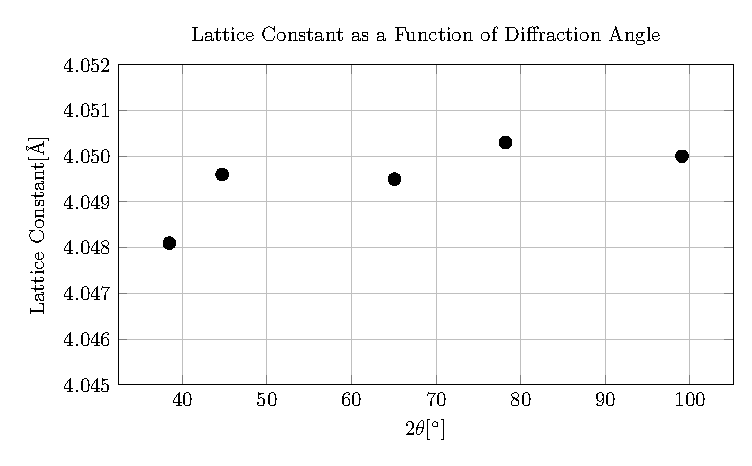
\includegraphics[width=0.7\columnwidth]{xrd_graph3.pdf}
            \caption{各ピークに対応する格子定数}
            \label{fig:lattice}
          \end{figure}
          $1/d^2$  vs.  $h^2+k^2+l^2$のグラフが\cref{fig:1/d}であり, このグラフを切片のある一次関数で近似したところ格子定数は4.0504\AA だった. 系統誤差の分析については考察で行った.
          \begin{figure}[H]
            \centering
            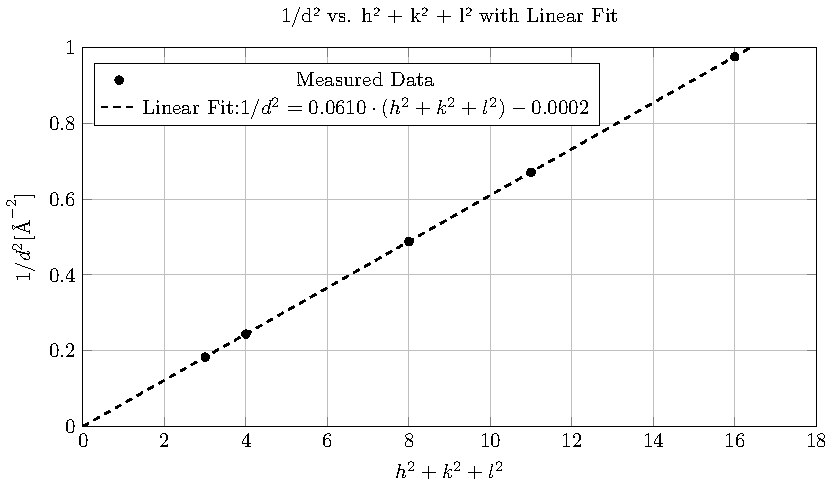
\includegraphics[width=0.7\columnwidth]{xrd_graph4.pdf}
            \caption{$1/d^2$ vs $h^2+k^2+l^2$と近似直線}
            \label{fig:1/d}
          \end{figure}
          格子定数と文献値の比較は考察で行った.
      \end{enumerate}
      各ピークから求めた格子定数の平均は4.0495\AA , 近似直線から求めた格子定数は4.0504\AA であった.
  \section*{考察}
    \subsection*{課題2.4}
      各ピークに対応する格子定数の系統誤差は見られなかった.\\
      残差のデータは\cref{fig:zansa}にプロットした. こちらにも系統誤差は見られなかった.\\
      今回切片の値は0.0002であった. 切片の値が0でない理由としては, PSD openingの値が$2.9397^\circ$と測定の刻みに対して大きかったことが考えられる. この値が大きいことで他の角度からの回折も検出して近似直線が原点からずれたと考えられる. \\
      \begin{figure}[H]
        \centering
        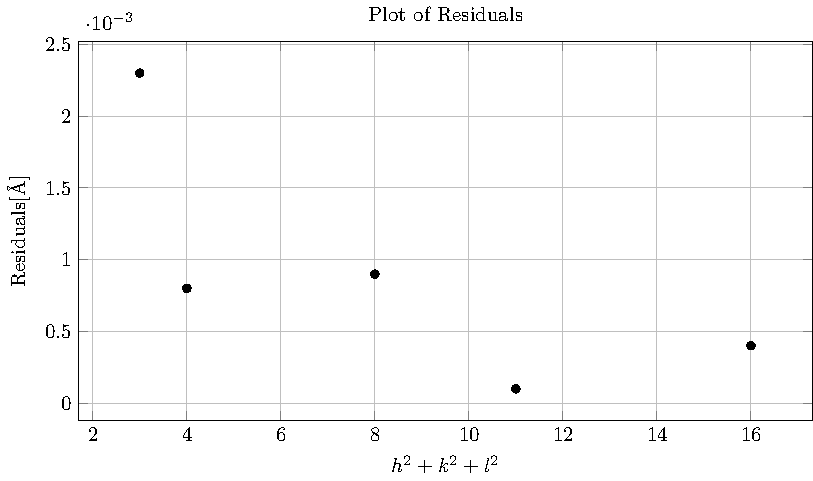
\includegraphics[width=0.7\columnwidth]{xrd_graph5.pdf}
        \caption{格子定数の測定値と近似曲線の残差}
        \label{fig:zansa}
      \end{figure}
      各ピークから求めた格子定数の平均は4.0495\AA , 近似直線から求めた格子定数は4.0504\AA だった. それぞれ文献値4.0496\AA との誤差は
      0.0024694\%,0.019755\%となり, 各ピークから導出した平均の方が誤差が小さかった. こうなった要因として近似直線に切片があったことが考えられる.
    \subsection*{課題3}
      \cref{tab:kaisetu},\cref{fig:kaisetu}にミラー指数の二乗和が4のときを1とした回折強度比を示した.\\
      これを見ると,ミラー指数の二乗和が3, つまり(1,1,1)のとき他の値に比べて大きくずれていることがわかる. この理由について, 測定に使用したAl板の結晶が粉末結晶のようにある反射面がランダムに配置されているわけではないのだと考えられる.\\
      このようになっている要因として, Al板の製造過程で圧延という工程を経ていることが考えられる. この工程である結晶面が発達し,または退化する. したがって回折強度比の測定値と理論値との間に差が出たのだと考えられる. 具体的には, (1,1,1)の面は大きく退化していることが考えられる.
      \begin{table}[H]
        \centering
        \begin{tabular}{|c|c|c|c|c|c|}\hline
          $h^2 + k^2 + l^2$&3&4&8&11&16\\\hline
          回折強度比(測定値)&0.050828&1&0.37003&0.91082&0.071749\\\hline
          回折強度比(理論値)&2.067503&1&0.63453&0.73500&0.444863\\\hline
        \end{tabular}
        \caption{回折強度比の比較}
        \label{tab:kaisetu}
      \end{table}
      \begin{figure}[H]
        \centering
        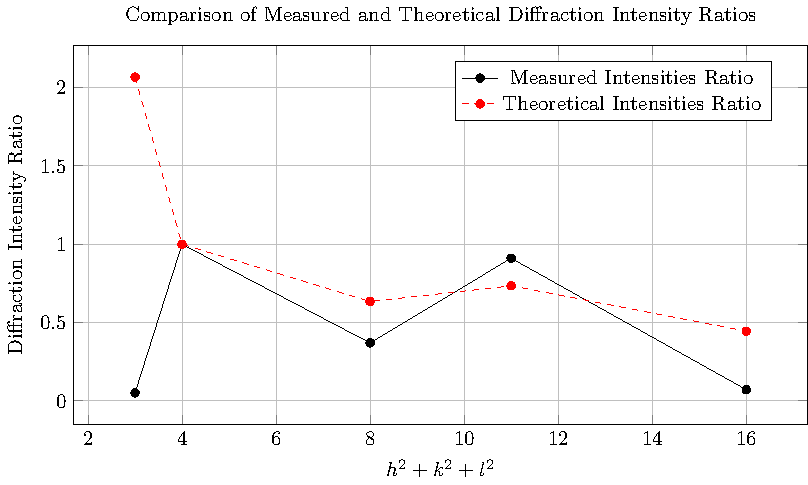
\includegraphics[width=0.7\columnwidth]{xrd_graph6.pdf}
        \caption{回折強度比の比較}
        \label{fig:kaisetu}
      \end{figure}
  \section*{まとめ}
    結晶の原子レベルの構造をX線回折を通して理解することができた.
  \section*{参考文献}
    \noindent 物理学総合実験テキスト X線回折\\
    日軽金アクト株式会社 アルミニウムの基礎データ https://group.nikkeikin.co.jp/act/technology/basic.html
\end{document}